\section{Artefact}\label{sec:artefact}
This section describes the created NetLogo model named `FoodDelivery'.
The file is available inside a git repository available at GitHub~\footnote{\url{https://github.com/evertvankammen/FooddeliveryNetlogo}}
This repository also contains Python code to automate running the model.

\subsection{Conceptional model}\label{subsec:conceptional-model}
The world that is being modelled is what is known as, the last mile in the food delivery industry.
This term is used for the last step in the delivery of online ordered goods.

Companies in the food delivery industry offer a service to three parties:
\begin{itemize}
    \item restaurants: they sell its food in a portal made by the delivery company.
    \item consumers: they buy food from a restaurant using the same portal.
    \item deliverers: they are steered by a mobile app also from the delivery company.
\end{itemize}

The steps in the food ordering and delivery proces are:
\begin{itemize}
    \item When a customer orders a meal, a message is sent to the restaurant.
    \item The restaurant starts preparing the meal, this may take some time (say on average 10 minutes).
    \item When it starts preparing, a deliverer is needed.
    \item A deliverer can claim the delivery (or is assigned) and starts cycling towards the restaurant.
    \item When the deliverer arrives at the restaurant it may have to wait until the meal is ready.
    \item When the meal is ready the deliverer takes it and start driving towards the customer.
    \item It may happen that no deliverer claims the meal, or it takes to long for the deliverer to get to the restaurant,
then the meal will be thrown away.
    \item If the meal gets delivered, the customer is happy
    \item If the meal is not delivered, the customer is unhappy.
    \item If a customer is unhappy it will eventually stop ordering meals.
\end{itemize}

This all takes place in a city where restaurants and customers are located.
The deliverers have to cycle to the restaurant and then to the customer.
The best route will be provided by the app the deliverers use.

The money for the delivery company is earned by charging the restaurants per delivery.
The companies interest is thus to have as many deliveries as possible.
This means they want to have happy customers and enough deliverers to keep them happy.

This is more or less how the process works in the real world.

Our model also has 3 types of agents:
-deliverers \\
-restaurants \\
-customers \\


The delivery company itself is not modelled, offers a website where customers can order,
restaurants pay the company a percentage of the delivery, they also offer means for the deliverers to
find deliveries and the shortest route.

Everything works on ticks of the clock, during 1 tick all agents execute one behavior rule.
The order of execution among agents of one type is arbitrary.
This is interleaved execution, no parallelism.


deliverers:
Start number can be set.
The deliverers get


restaurants:
the start number can be set, are placed at random
accept any orders, are open all the time,
prepare meals, the preparation time can be set,
after accepting a deliverer is asked.
when the meal is ready it can be picket up.
Restaurants will leave the system if they have not enough orders.

customers:
order distribution, peek ours breakfast, lunch and  diner, once a week.
order from any restaurant they have no bad experience with
the price distribution, average can be set
they remember bad experiences for a certain time.
If delivered stale the customer is not satisfied and will not order from the restaurant also
it will order less food per week.

\begin{figure}
    \centering
    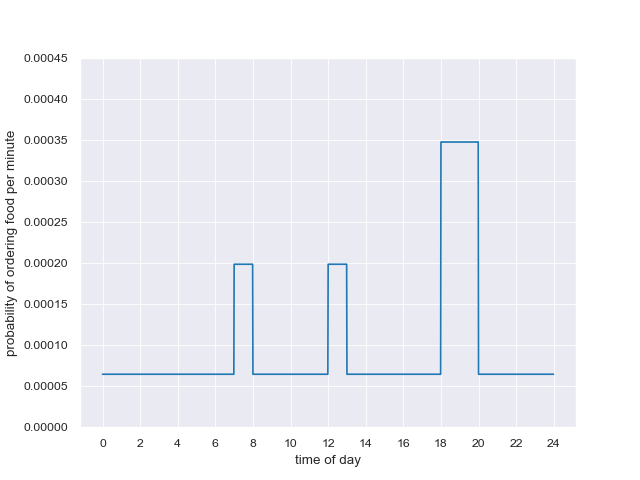
\includegraphics[width=8.5cm]{sections/pics/food_ordering_distribution}
    \caption{Food ordering probablities for one day}
    \label{fig:food_ordering_distribution}
\end{figure}



meals:
meals have properties, stage: ordered , ready, in\_transit, delivered, expired
A meal is only fresh for a time period.
If not picked up it wil be discarded.





\begin{itemize}
    \item   The world consists op a grid of squares, some squares will be blocks of buildings and others represent the streets.
    \item   On this grid some predetermined restaurants and customers exist.
    \item   Customers will order food at a restaurant, the restaurant will prepare the food en will ask for a deliverer.
    \item   A deliverer will claim the delivery, move to the restaurant, pick the food up and move to the customer.
    \item   Agents may leave the world, i.e.,choose another delivery company, when unhappy.
    \item   Unhappiness will occur:
    \begin{itemize}
        \item   for customers when the food is not or too late delivered,
        \item   for restaurants when the food is not picked up or no orders are being placed,
        \item   for deliverers when they don't make any money.
    \end{itemize}
    \item    Calculating the profit for the delivery company.
    \item    The simulation consists of discreet steps, in which all agents simultaneous can do one thing.
    Some examples are:
    \begin{itemize}
        \item  move to the next square
        \item  place an order at a restaurant
        \item  do nothing
        \item  decide to take an order
    \end{itemize}
    \item   Behavior of the agents is rule based, these have to be programmed.
\end{itemize}


The environment where multiple agents act is called a multi-agent system end the problem is called a multi-agent planning problem (from~\cite{russell2016artificial}).
The research problem is actually a comparison between a system where there is one decision maker (the company assigns delivery jobs) and a system where each deliverer decide for its self (multiple decision makers).
This research will not be of a thoroughly theoretical nature though, its more of an exploratory/explanatory nature, see what happens under some conditions and explain the correlation.

\subsection{Computer model}\label{subsec:computer-model}

\begin{figure}
    \centering
    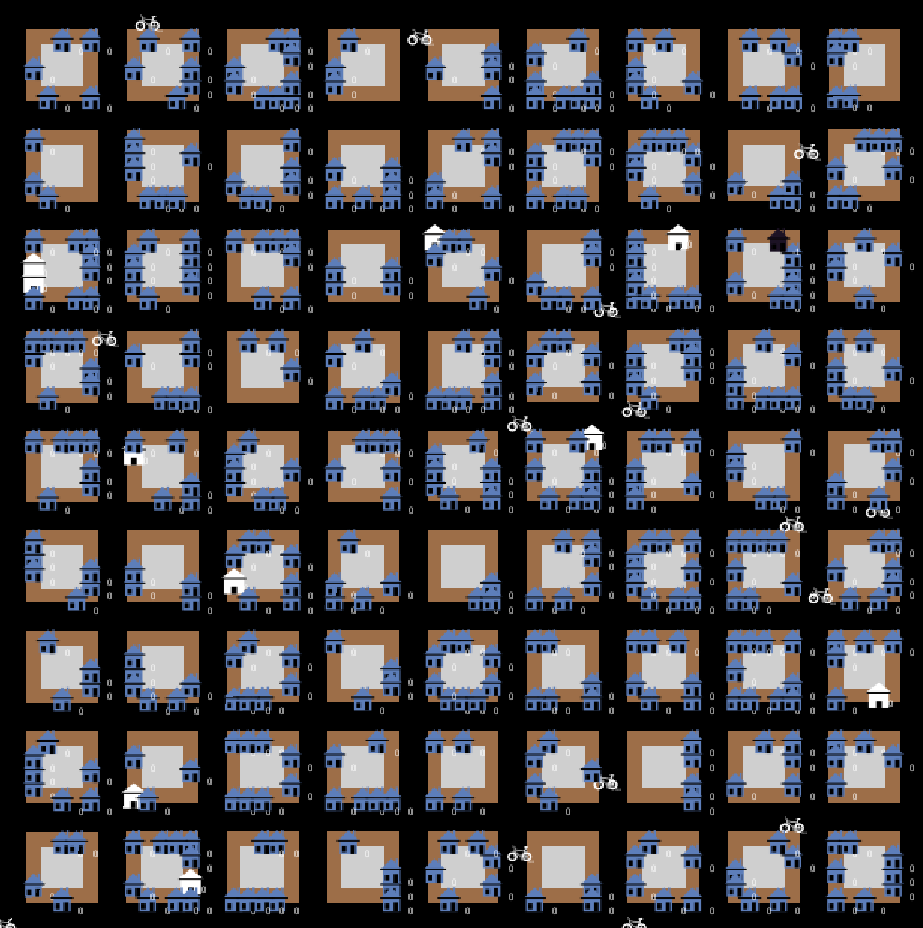
\includegraphics[width=8.5cm]{sections/pics/grid}
    \caption{Fooddelivery grid}
    \label{fig:grid}
\end{figure}

\begin{figure}
    \centering
    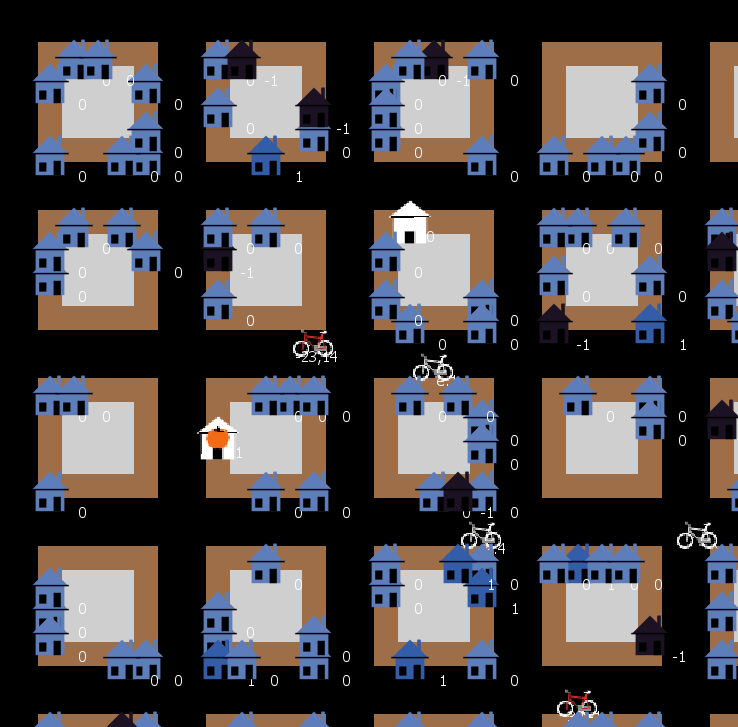
\includegraphics[width=8.5cm]{sections/pics/grid_closeup}
    \caption{Fooddelivery grid closeup}
    \label{fig:grid closeup}
\end{figure}


\begin{figure}
     \centering
     \begin{subfigure}[m]{0.1\textwidth}
         \centering
         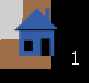
\includegraphics[width=\textwidth]{sections/pics/cust_happy}
         \caption{Customer with happyness score}
     \end{subfigure}
     \hfill
     \begin{subfigure}[m]{0.1\textwidth}
         \centering
         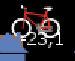
\includegraphics[width=\textwidth]{sections/pics/del_on_its_way}
         \caption{Deliverer on route to loc 23,1}
     \end{subfigure}
     \hfill
     \begin{subfigure}[m]{0.1\textwidth}
         \centering
         
\includegraphics[width=\textwidth]{sections/pics/meal_prep}
         \caption{Restaurant with meal ordered on top and number of ordered}
     \end{subfigure}
      \hfill
     \begin{subfigure}[m]{0.1\textwidth}
         \centering
         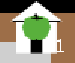
\includegraphics[width=\textwidth]{sections/pics/meal_ready}
         \caption{Restaurant with meal ready on top and number of ordered}
     \end{subfigure}
        \caption{Agents examples}
        \label{fig:agents}
\end{figure}






\section{Results of simulations}\label{sec:results-of-simulations}


Consumers order meals from restaurants they like, if a meal is delivered cold they dislike the restaurant.
If they dont like the restaurant they will not place any orders anymore at that restaurant.

Restaurants create meals, if they dont get any orders for some time they quit.

The delivery provider make money for each order placed via their system, at the end they must have enough deliverers so that
customers keep ordering.
They have to pay the deliverers for the deliveries.



\subsection{Model variant 1}
Here come the results belonging to variant where deliverers are hired and paid an hourly wage.
The company destributes deliveries equally among the hired employees.
The company has to deside on how many to hire and for which periods.


\subsection{Model variant 2}
Here come the results where deliverers are independent contractors.
Deliverers come and go whenever they are pleased, like a open market.
Now deliverers have to deside to become a deliverer, deside to stop and to decide to go for a delivery.
To keep this simple, the meals are destributed among the available deliverers.
If a delivery person does not make enough many during a day they will quit.
